\documentclass[12pt]{article}
\usepackage[left=0.25cm,top=1cm,right=0.25cm,bottom=1cm]{geometry}
\textwidth = 20cm
\hoffset = -1cm
\usepackage[utf8]{inputenc}
\usepackage[spanish,es-tabla]{babel}
\usepackage[autostyle,spanish=mexican]{csquotes}
\usepackage[tbtags]{amsmath}
\usepackage{nccmath}
\usepackage{amsthm}
\usepackage{amssymb}
\usepackage{graphicx}
\usepackage{standalone}
\usepackage[outdir=./]{epstopdf}
\usepackage{siunitx}
\usepackage{physics}
\usepackage{color}
\usepackage{float}
\usepackage{multicol}
%\usepackage{milista}
\usepackage{enumitem}
\usepackage{anyfontsize}
\usepackage{anysize}
\usepackage{enumitem}
\usepackage{capt-of}
\usepackage{bm}
\usepackage{relsize}
\usepackage{placeins}
\usepackage{empheq}
\usepackage{cancel}
\usepackage{wrapfig}
\spanishdecimal{.}
\renewcommand{\baselinestretch}{1.5} 
\renewcommand\labelenumii{\theenumi.{\arabic{enumii}}}
\newcommand{\ptilde}[1]{\ensuremath{{#1}^{\prime}}}
\newcommand{\stilde}[1]{\ensuremath{{#1}^{\prime \prime}}}
\newcommand{\ttilde}[1]{\ensuremath{{#1}^{\prime \prime \prime}}}
\newcommand{\ntilde}[2]{\ensuremath{{#1}^{(#2)}}}


\title{Transformada de Fourier \\ \Large{Ejercicios}} \vspace{-3ex}
\author{M. en C. Gustavo Contreras Mayén}
\date{ }
\newcommand{\Cancel}[2][black]{{\color{#1}\cancel{\color{black}#2}}}
\begin{document}
\vspace{-4cm}
\maketitle
\fontsize{14}{14}\selectfont
\tableofcontents
\newpage

\section{La Transformada de Fourier.}
\subsection{Áreas de aplicación.}

Las aplicaciones de la Transformada de Fourier (TF) son muy extensas, ya que abarcan diversas ramas de la física matemática.
\par
Desde la teoría de números y geometría hasta óptica y mecánica cuántica, así como otras áreas de la ciencia tales como: la medicina, comunicaciones, ingeniería biomédica, ingeniería mecánica y de control, campos electromagnéticos, procesamiento de señales de audio y procesamiento de imágenes.
\par
La TF también se utiliza para:
\begin{enumerate}
\item Analizar contenido de frecuencia de las señales.
\item Determinar como cambia la amplitud y las fases de las señales sinusoidales cuando éstas pasan a través de un sistema lineal e invariante en el tiempo.
\item Generar formas de onda de corriente o tensión eléctrica por medio de la superposición de señales senoidales generadas por osciladores electrónicos de amplitud variable cuyas frecuencias ya están determinadas.
\item Analizar el comportamiento armónico de una señal.
\end{enumerate}

\subsection{Ejemplos concretos.}


En el campo del electromagnetismo y de microondas, la Transformada de Fourier está relacionada con:
\begin{itemize}
\item El cálculo del campo cercano transitorio que es irradiado por dispositivos electrónicos.
\item El análisis de fenómenos ópticos en microondas.
\item El cálculo del campo electromagnético de rayos, la formación de haz y la radiación de microondas solares.
\end{itemize}

En Medicina, el análisis de la TF está relacionado con:
\begin{itemize}
\item El análisis espectral del comportamiento global de los cromosomas.
\item El análisis espectral de la variabilidad de la frecuencia cardíaca.
\item El procesamiento de imágenes generadas por econogramas, resonancias magnéticas y tomografía axial.
\end{itemize}

En el área de comunicaciones se usa para:
\begin{itemize}
\item Analizar la frecuencia de señales.
\item Diseñar los sistemas de transmisión de señales para transmitir información.
\item Diseñar supresores y canceladores de ecos en líneas telefónicas.
\end{itemize}

En el campo de la ingeniería mecánica:
\begin{itemize}
\item  Se utiliza para balancear rotores y eliminar la vibración que se genera cuando no están balanceados.
\item Estudiar los problemas relacionados con vibraciones mecánicas en los motores, generadores y equipos rotatorios en general.
\end{itemize}

En el procesamiento de señales de audio:
\begin{itemize}
\item Se usa para compactar las señales de audio (formatos MP3 y MP4).
\item Producir efectos de sonido, diseñar sintetizadores de audio y ecualizadores.
\end{itemize}

En un campo extendido del procesamiento de imágenes:
\begin{itemize}
\item La TF se utiliza para filtrar imágenes, extraer características de interés.
\item Realizar transformaciones de imágenes y compactar imágenes.
\end{itemize}

Algo de lo que podemos hacer con la TF de una imagen es eliminar algunos componentes.
\par
Si eliminamos las frecuencias bajas, menores de cierto valor $\omega_{f}$, se le llama \textbf{filtro de paso alto}.  Una gran cantidad de ruido de fondo se produce a bajas frecuencias, por lo que un filtro de paso alto puede limpiar una señal.
\par
Si descartamos las frecuencias altas, se llama \emph{filtro de paso bajo}. Se puede usar un filtro de paso bajo para suavizar los datos (como una foto digital), ya que arroja ruido de alta frecuencia.
\par
Un filtro que corta las frecuencias altas y bajas se llama \emph{filtro de paso de banda}.

A continuación veremos un ejemplo\footnote{En el software para manejo de imágenes como Photshop, GIMP, Picasa, etc. se cuenta con un conjunto de filtros que modifican la apariencia de una imagen, ya sea con la finalidad de corregir detalles o mejorar la misma; básicamente se están utilizando transformadas de Fourier, pero no se le llaman de esta manera, sino que le dan otros nombres comercialmente más atractivos dentro del software.} de la aplicación de un filtro pasa altos en una imagen, a la izquierda tenemos la imagen original, mientras que a la derecha la imagen resultante luego de ocupar el filtro pasa altos:
\begin{figure}[H]
    \centering
    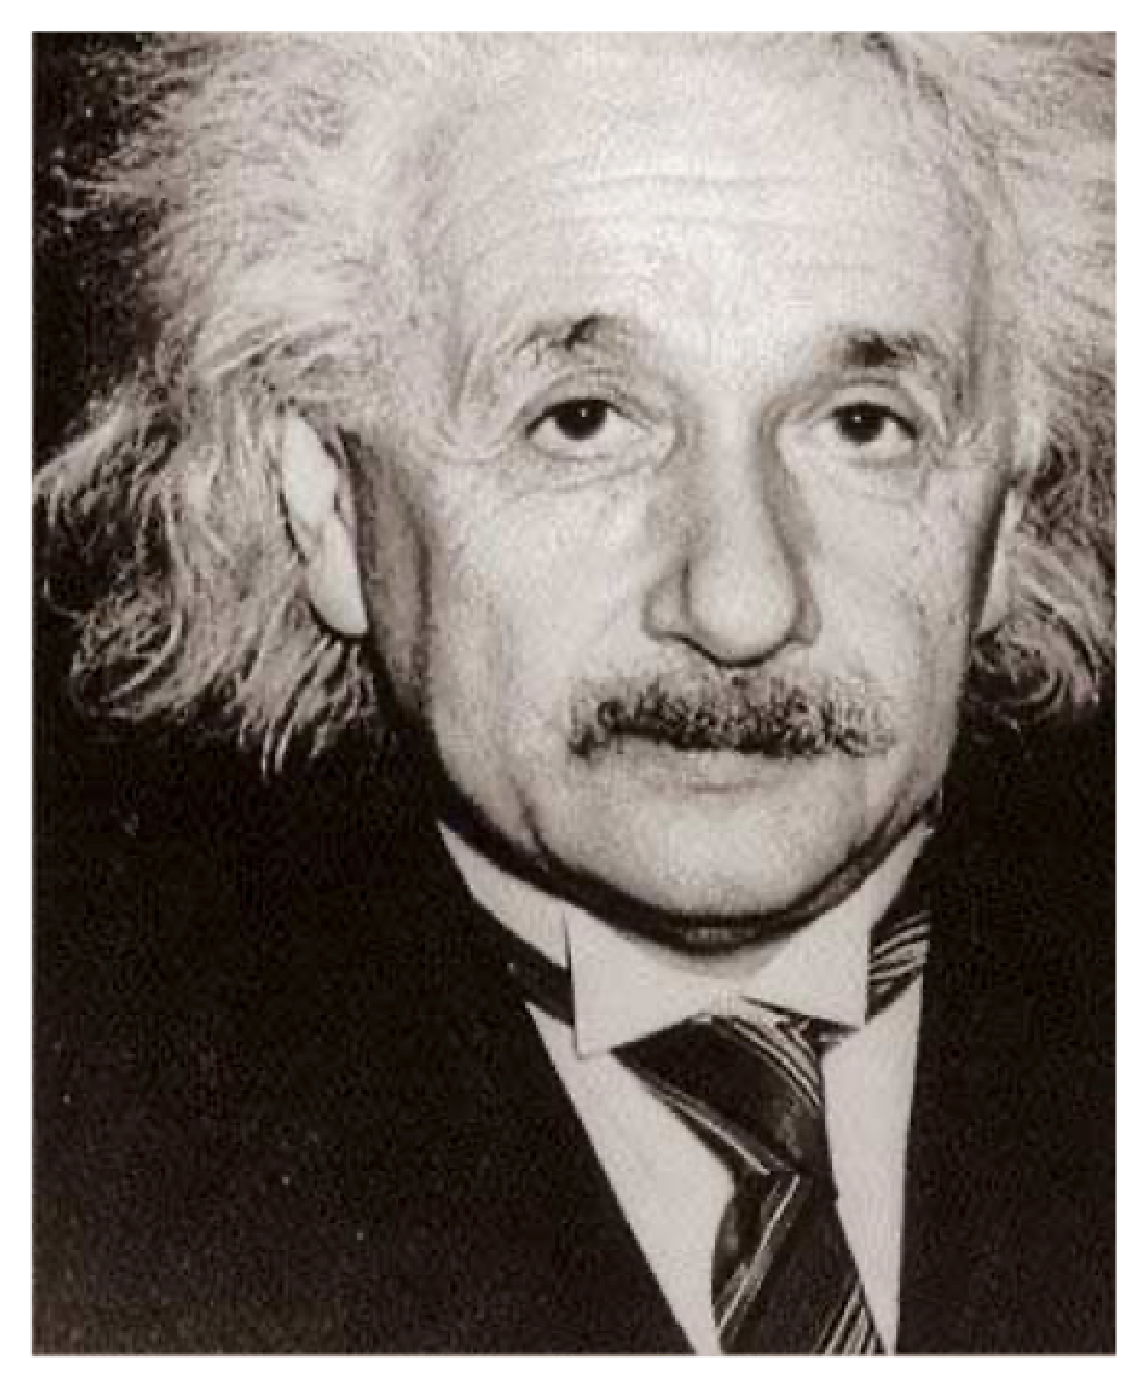
\includegraphics[scale=0.35]{Imagenes/Einstein_01.eps}
    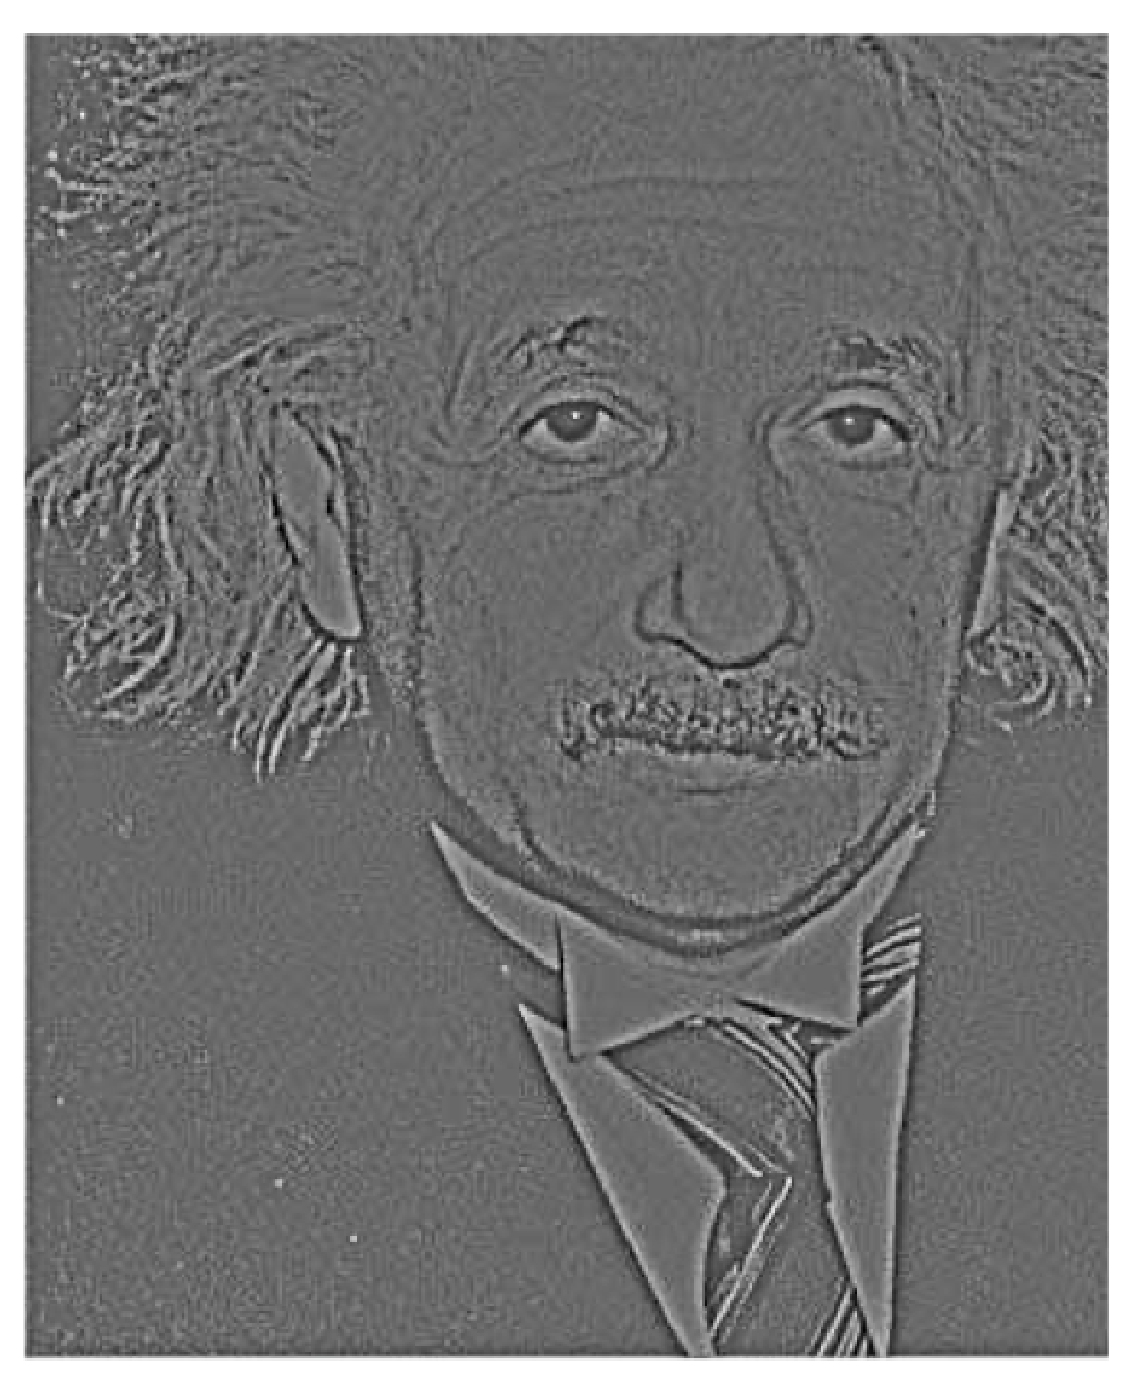
\includegraphics[scale=0.35]{Imagenes/Einstein_02.eps}
\end{figure}

En el siguiente ejemplo se presenta la aplicación de un filtro pasa bajos sobre otra imagen, nuevamente a la izquierda se presenta la imagen original y a la derecha, la imagen resultante luego de ocupar el filtro:
\begin{figure}
    \centering
    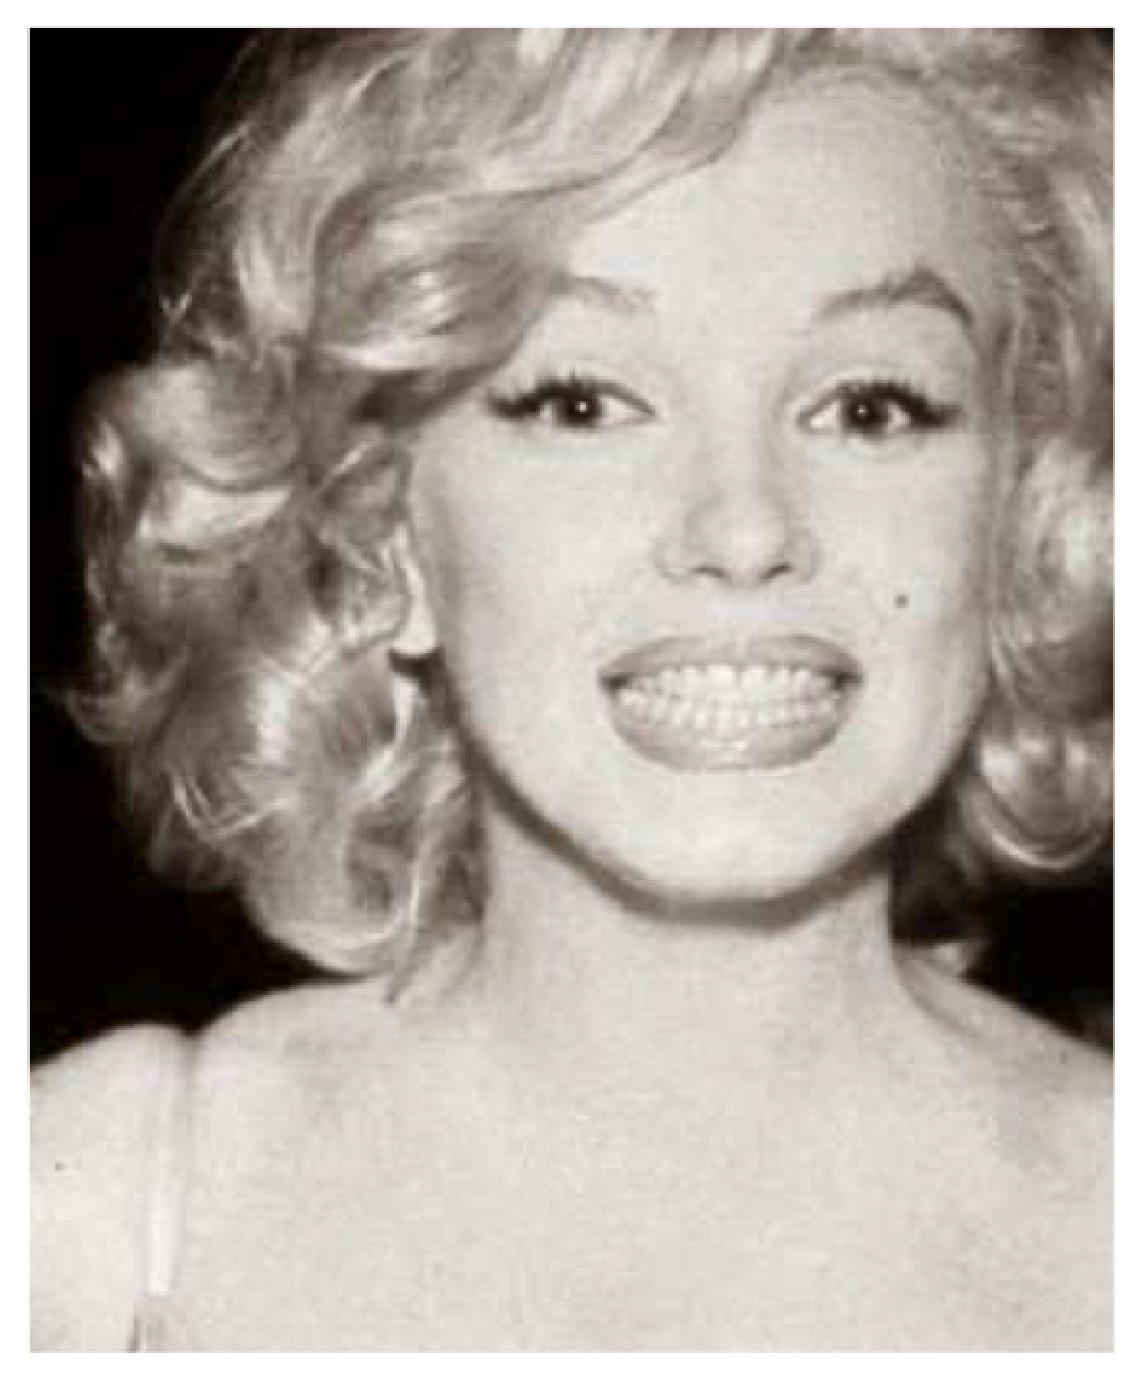
\includegraphics[scale=0.35]{Imagenes/Marylin_01.eps}
    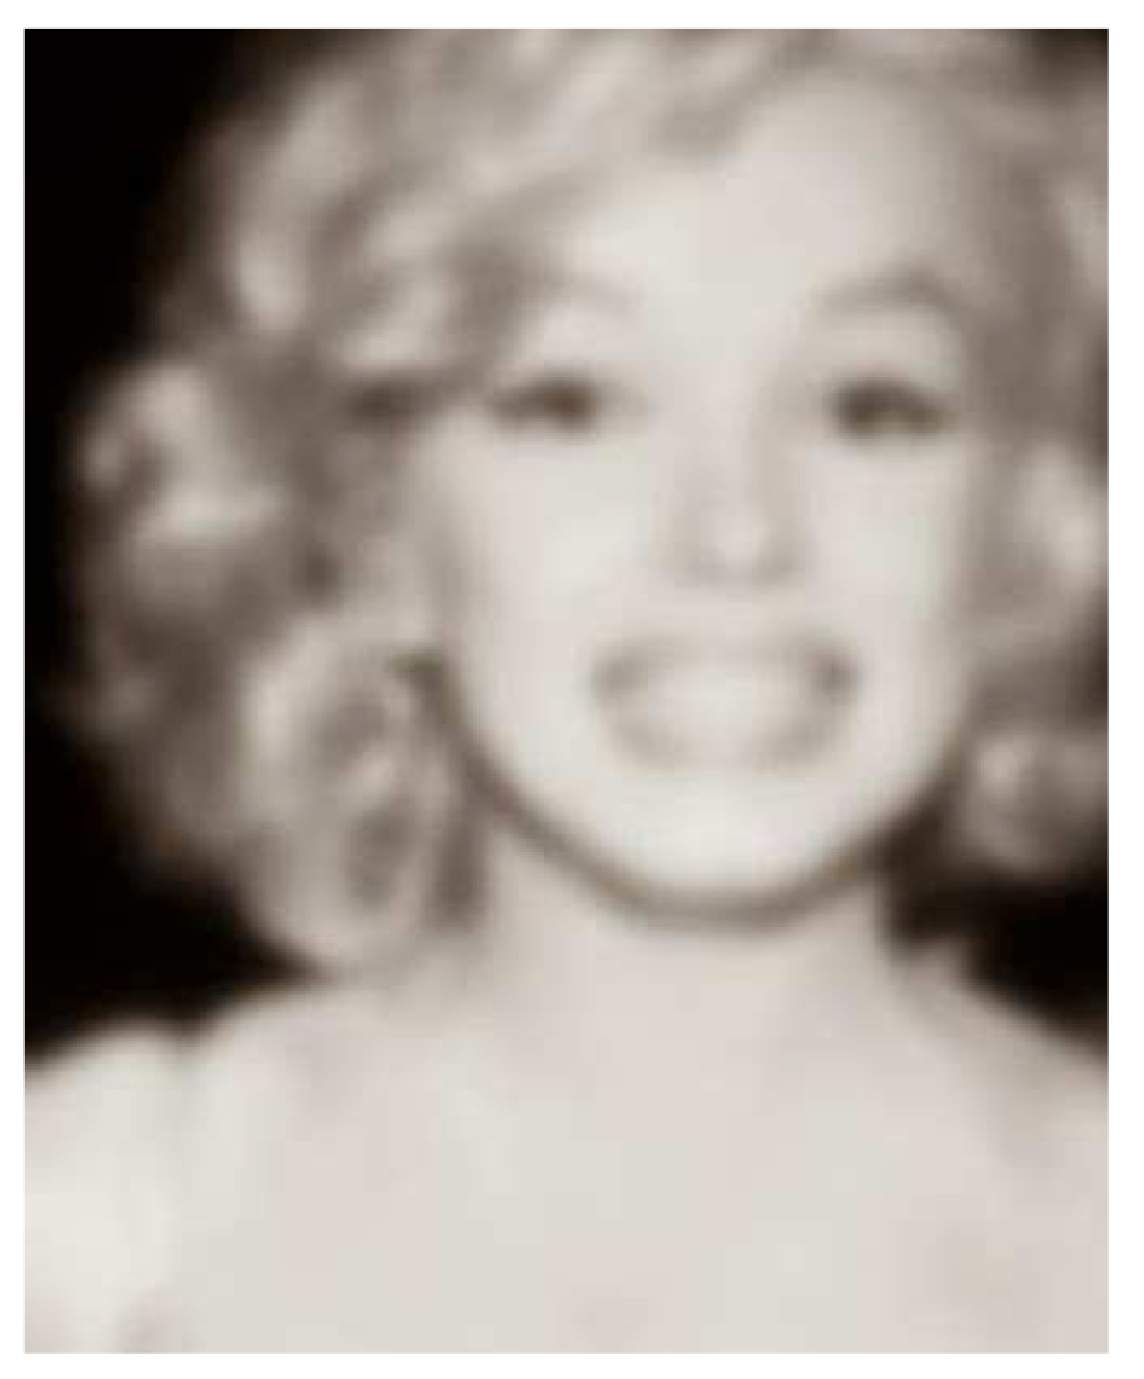
\includegraphics[scale=0.35]{Imagenes/Marylin_02.eps}
\end{figure}

Veamos que el resultado obtenido \enquote{desenfoca} la imagen original.
\par
Si combinamos los filtros pasa alto en la imagen de Einstein y el filtro pasa bajo en la imagen de Marylin, obtenemos:
\begin{figure}[H]
    \centering
    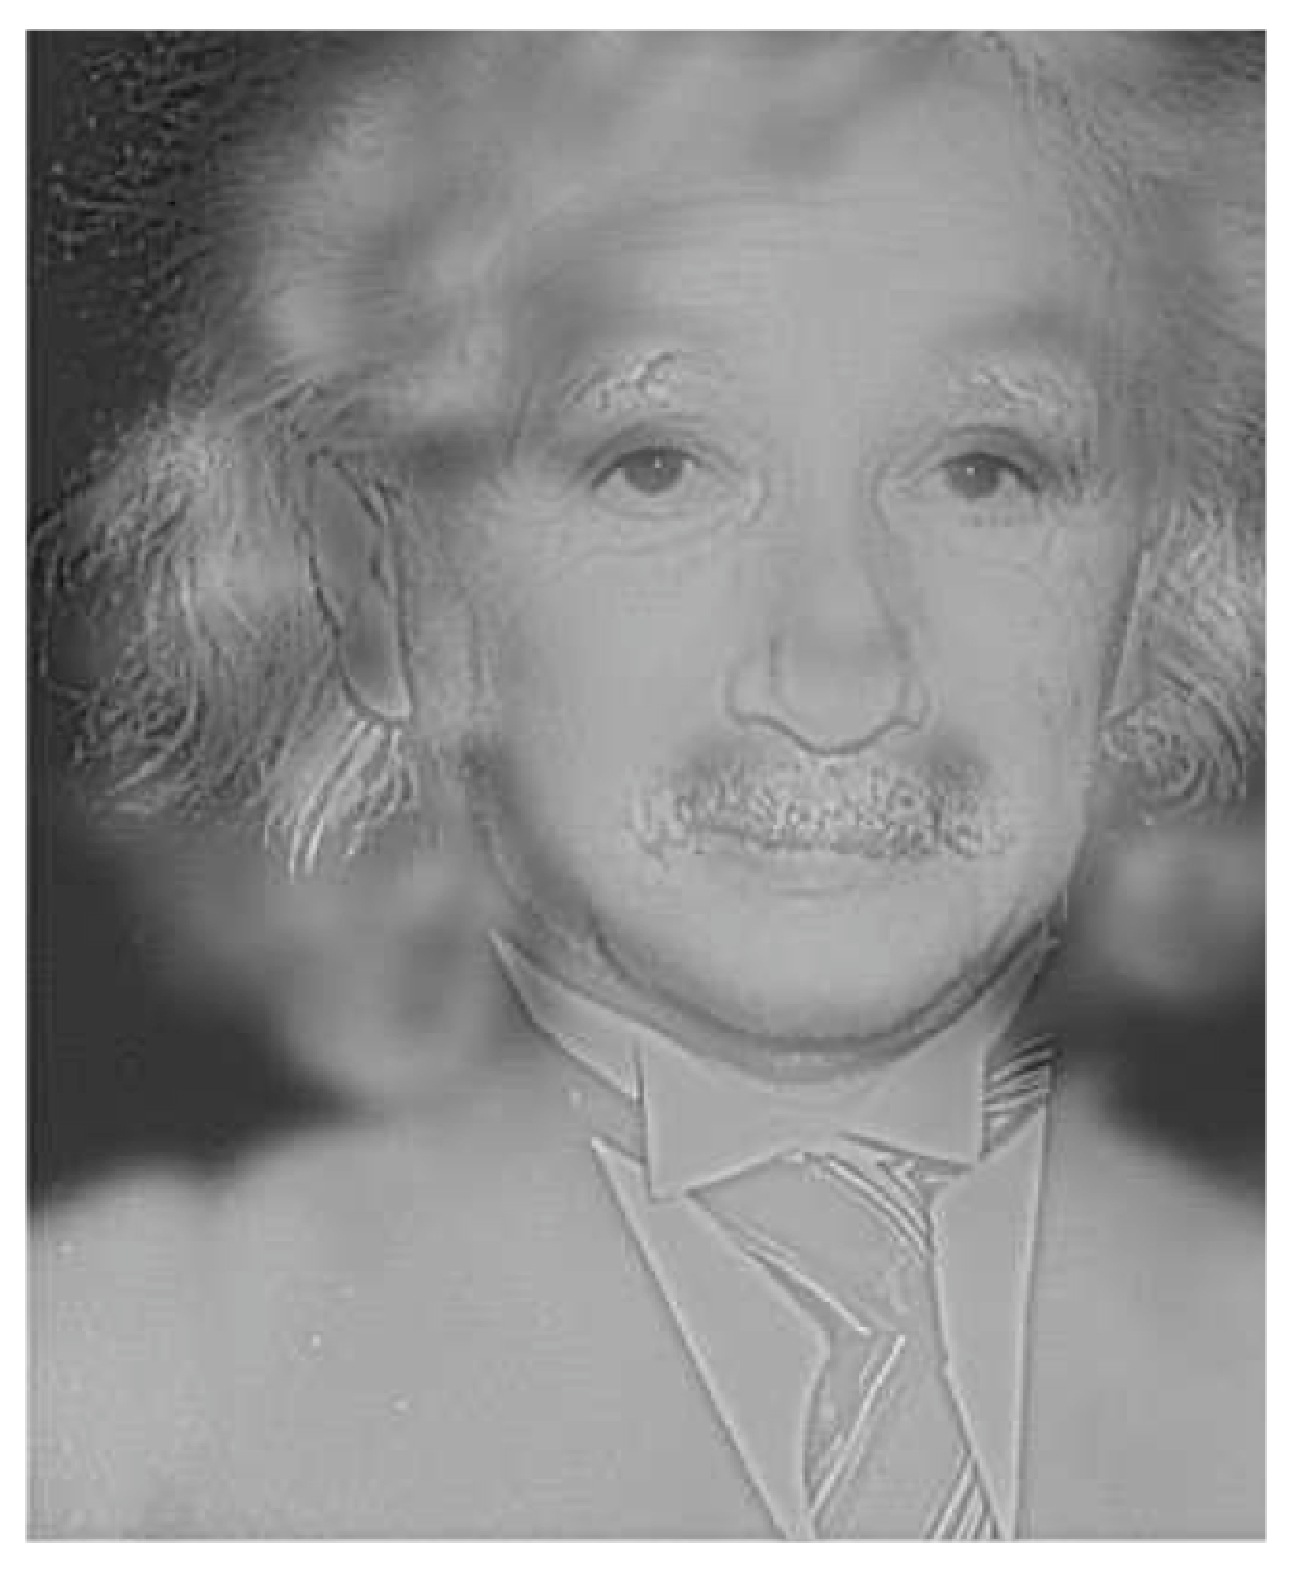
\includegraphics[scale=0.35]{Imagenes/Einstein_Marylin_AB_01.eps}
    \caption{Filtro pasa alto Einstein + pasa bajo Marylin}
    \label{fig:figuraEpa_Mpb}
\end{figure}
Notamos una superposición de las dos imágenes, curiosamente si nos acercamos a la imagen, nuestro cerebro procesa la información que recibe y perfila a uno de los dos personajes, mientras que si nos alejamos de la imagen, reconocemos al otro personaje.
\par
Hacemos el cambio de filtros: en la imagen de Einstein se ocupa el filtro pasa bajo y en la imagen de Marylin, se ocupó el filtro pasa altos:
\begin{figure}[H]
    \centering
    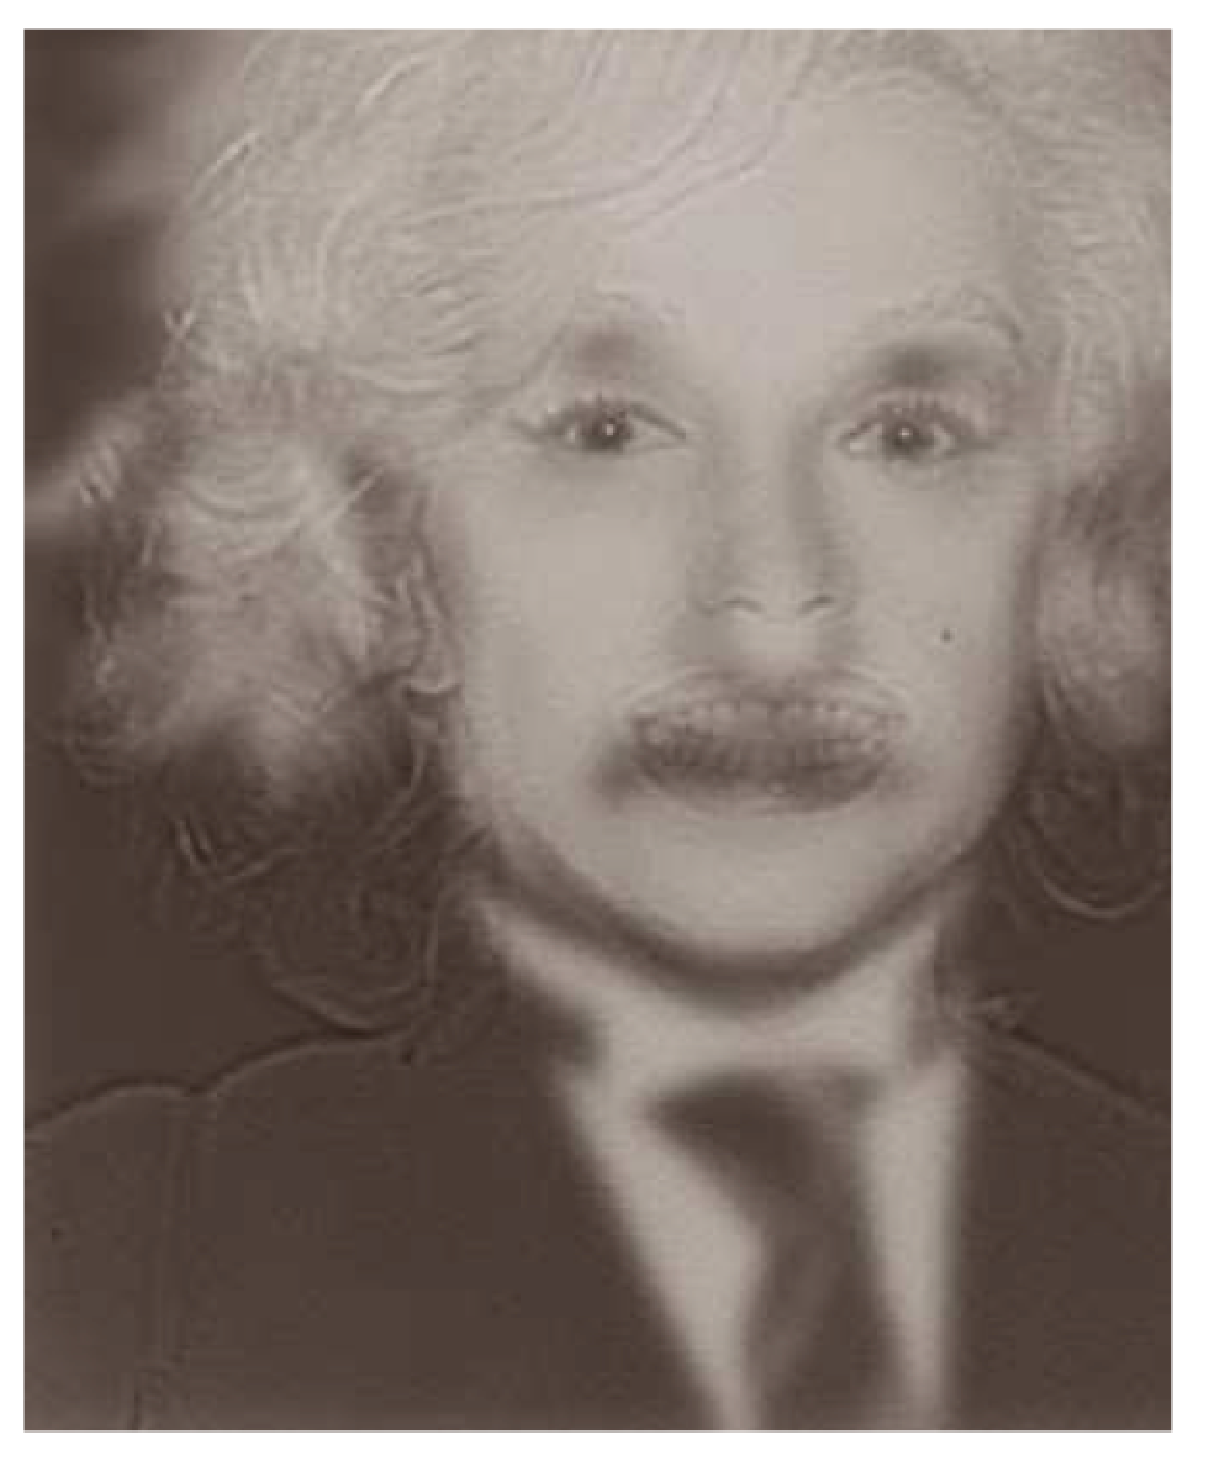
\includegraphics[scale=0.35]{Imagenes/Einstein_Marylin_BA_01.eps}
    \caption{Filtro pasa bajo Einstein + pasa alto Marylin}
\end{figure}

¿Será que al invertir los filtros en las imágenes, ahora el personaje que se reconoce cuando nos acercamos es el contrario que en el caso de la imagen de la figura (\ref{fig:figuraEpa_Mpb})?

\section{Transformada de Fourier.}

\subsection{Definición.}

Se define la transformada de Fourier como:
\begin{align}
F \big[ f(x); x \to \xi \big] = \dfrac{1}{\sqrt{2 \, \pi}} \scaleint{5ex}_{\bs -\infty}^{+\infty} f(x) \, \exp(i \, \xi \, x) \dd{x}
\label{eq:ecuacion_01_12}
\end{align}

Mientras que la transformada inversa de Fourier se define de la siguiente manera:
\begin{align}
f(x) = F^{-1} \big[ F(\xi) \big] = \dfrac{1}{\sqrt{2 \, \pi}} \int_{-\infty}^{+\infty} F(\xi) \, \exp(-i \, \xi \, x) \dd{\xi}
\label{eq:ecuacion_01_13}
\end{align}
en un punto continuo de $f(x)$.

Recuerden que el detalle de las propiedades de la Transformada de Fourier se indican en las notas de trabajo, por lo que esperamos que las hayan revisado de manera oportuna.

\subsection{Ejercicios con la Transformada de Fourier.}

\subsection*{Primer ejercicio.}

Evalúa la transformada de Fourier de:
\begin{align*}
f(x) = \begin{cases}
x, & \abs{x} < a \\
0, & \abs{x} > a
\end{cases}
\end{align*}

Ocupamos la definición de la transformada de Fourier, que se indica en la ec. (\ref{eq:ecuacion_01_12}), así que:
\begin{align*}
F \big[ f(x); x \to \xi \big] = \dfrac{1}{\sqrt{2 \, \pi}} \scaleint{5ex}_{\bs -a}^{a} x \, \exp(i \, \xi \, x) \dd{x}
\end{align*}

Resolvemos la integral por partes\footnote{Para abreviar el material de trabajo, se presentan los resultados, pero pueden realizar a mano todo el trabajo y corroborar que lo que mostramos es correcto.}, y obtenemos lo siguiente:
\begin{align*}
&= \dfrac{1}{\sqrt{2 \, \pi}} \left\{ \bigg[ x \, \dfrac{\exp(i \, \xi \, x)}{i \, \xi} \bigg] \bigg\vert_{-a}^{a} - \dfrac{1}{i \, \xi} \scaleint{5ex}_{\bs -a}^{a} \exp(i \xi \, x) \dd{x} \right\} \\[1em] 
&= \dfrac{1}{\sqrt{2 \, \pi}} \bigg[ \dfrac{a \, e^{i \xi a} + a \, e^{-i \xi a}}{i \, \xi} + \dfrac{1}{\xi^{2}} \left( e^{i a \xi} - e^{-i a \xi} \right) \bigg] =
\end{align*}

Ocupando las identidades de Euler conocidas, en donde se relacionan las funciones trigonométricas, con la función exponencial, se tiene que:

\begin{align*}
&= \dfrac{1}{\sqrt{2 \, \pi}} \bigg[ \dfrac{2 \, a \, \cos a \xi}{i \, \xi} + \dfrac{2 \, i \, \sin a \xi}{\xi^{2}} \bigg] = \\[1em] 
&= \sqrt{\dfrac{2}{\pi}} \, i \, \bigg[ \dfrac{\sin a \xi - a \, \xi \, \cos a \, \xi}{\xi^{2}} \bigg]
\end{align*}

\subsection*{Segundo ejercicio.}

Calcula la transformada de Fourier de:
\begin{align*}
f(x) = \exp(-a \, \abs{x}), \hspace{1cm} a > 0
\end{align*}

Ocupamos nuevamente la definición de la TF, por lo que:
\begin{align*}
F \big[ f(x); x \to \xi \big] {=} \dfrac{1}{\sqrt{2 \pi}} \scaleint{5ex}_{\bs -\infty}^{+\infty} \exp(-a \abs{x}) \, \exp(i \xi x) \dd{x}
\end{align*}
Para resolver la integral, primero \enquote{separamos} en el dominio el integrando:
\begin{align*}
= \dfrac{1}{\sqrt{2 \pi}} \bigg[ \scaleint{5ex}_{\bs -\infty}^{0} e^{ a  x} \, e^{i \xi x} \dd{x} + \scaleint{5ex}_{\bs 0}^{\infty} e^{ -a  x} \, e^{i \xi x} \dd{x} \bigg] =
\end{align*}

Cada integral se resuelve directamente y se evalúa en los límites de integración, notemos que al tener en el integrado el producto de funciones exponenciales, ocupamos las propiedades de la misma, por lo que se simplifica la expresión y el cálculo de la integral es a la vez, más sencillo. Se obtiene entonces:
\begin{align*}
&= \dfrac{1}{\sqrt{2 \pi}} \bigg[ \dfrac{1}{a + i \, \xi} + \dfrac{1}{a - i \xi} \bigg] = \\[0.5em] 
&= \sqrt{\dfrac{2}{\pi}} \, \dfrac{a}{a^{2} + \xi^{2}}
\end{align*}

%REf. Zill Cap. 7.4 Transformada de Fourier Ejemplo 2
\section{Ecuación de calor.}
\subsection{Temperatura en una placa semiinfinita.}


La temperatura constante de una placa semiinfinita está dada por la siguiente ecuación diferencial, condiciones iniciales y de frontera:
\begin{align*}
&\pdv[2]{u}{x} + \pdv[2]{u}{y} = 0 \hspace{1cm} 0 < x < \pi, \hspace{0.3cm} y > 0 \\[0.5cm]
&u(0, y) = 0 \hspace{1cm} u(\pi, y) = e^{-y} \hspace{0.3cm} y > 0 \\[0.5cm]
&\pdv{u}{y} \eval_{y=0} = 0 \hspace{1cm} 0 < x < \pi
\end{align*}

El problema a resolver en este ejercicio es: \textbf{Encuentra el valor de temperatura de $u(x,y)$}.

\begin{figure}[H]
    \centering
    \includegraphics[scale=1.3]{Imagenes/Transformada_Fourier_Placa_Ejemplo.eps}
    \caption{Placa semiinfinita con las condiciones iniciales que determina el problema.}
\end{figure}

El dominio de la variable y la condición prescrita en $y = 0$, indican que se puede aplicar la transformada coseno de Fourier al problema, definimos así:
\begin{align*}
F_{c} \big[u(x,y)\big] = \scaleint{5ex}_{\bs 0}^{\infty} u(x, y) \, \cos \alpha \, y \dd{y} = U(x, \alpha)
\end{align*}


Como la transformada coseno de Fourier de la derivada de una función es:
\begin{align*}
F_{c} \big[\stilde{y}(x)] = - \alpha^{2} \, F[\alpha] - \ptilde{f} (0)
\end{align*}
se tiene que:
\begin{align*}
F_{c} \left[\pdv[2]{u}{x} \right] + F_{c} \left[\pdv[2]{u}{y} \right] = F_{c} [0]
\end{align*}
Por lo tanto:
\begin{align*}
\dv[2]{U}{x} - \alpha^{2} \, &U(x, \alpha) - u_{y} (x, 0) = 0 \\[1em]
&\Rightarrow \hspace{0.3cm} \dv[2]{U}{x} - \alpha^{2} \, U = 0
\end{align*}
Recordemos que $(\pdv*{u}{y})\eval_{y=0} = 0$, la EDO2H es una ecuación que ya sabemos resolver, se muestra el resultado a continuación.
\\[0.5em]
Puesto que el dominio de $x$ es un intervalo finito, es preferible escribir la solución a la EDO como:
\begin{align}
U(x, \alpha) = c_{1} \, \cosh (\alpha \, x) + c_{2} \, \sinh (\alpha \, x)
\label{eq:ecuacion_016}
\end{align}

Ahora bien, las transformadas de Fourier en los puntos $x = 0$ y $x = \pi$, son:
\begin{align*}
F_{c} \big[ u(0, y)\big] &= F_{c} [0] \\[0.5em]
F_{c} \big[ u(\pi, y)\big] &= F_{c} \big[ e^{-y} \big]
\end{align*}
y son equivalentes a:
\begin{align*}
U(0, \alpha) &= 0 \\[0.5em]
U(\pi, \alpha) &= \dfrac{1}{1 +  \alpha^{2}}
\end{align*}
respectivamente.

Cuando se aplican estas últimas condiciones, en la solución ec. (\ref{eq:ecuacion_016}) nos devuelve el valor de los coeficientes:
\begin{align*}
c_{1} &= 0 \\[0.5em]
c_{2} &= \dfrac{1}{(1 + \alpha^{2}) \, \sinh \alpha \pi}
\end{align*}
Por lo tanto, la transformada coseno de Fourier es:
\begin{align*}
U(x, \alpha) = \dfrac{\sinh \alpha \, x}{(1 + \alpha^{2}) \, \sinh \alpha \pi}
\end{align*}

De modo que al ocupar la transformada coseno inversa de Fourier, tenemos que:
\begin{align*}
F_{c}^{-1} \big[F(\alpha)\big] = \dfrac{2}{\pi} \scaleint{5ex}_{\bs 0}^{\infty} F[\alpha] \, \cos \alpha \, x \dd{x}
\end{align*}

Para obtener el siguiente resultado que nos determina la solución $u(x,y)$ en los puntos dentro de la placa semiinfinita:
\begin{align*}
u(x, y) = \dfrac{2}{\pi} \scaleint{6ex}_{\bs 0}^{\infty} \dfrac{\sinh \alpha \, x}{(1 + \alpha^{2}) \, \sinh \alpha \pi} \, \cos \alpha \, x \dd{x}
\end{align*}
La solución obtenida se le conoce como \emph{solución fundamental}.

\end{document}